\chapter{Marco teórico}
\label{Marco_teorico}

Cuando uno busca desarrollar un producto es una buena práctica el investigar que se ha realizado
previamente en entregas similares, ver que ténicas se han utilizado y que problemas se han
encontrado y como los solventaron. También es interesante ver que mecánicas se han ido consevando
y que innovaciones se han ido introduciendo con el paso del tiempo.

A continuación vamos a detallar aspectos de interés encontrados en diversas entregas
las cuales nos servirán de referentes.

\section{Age of Empires II: The Age of Kings}
En primer lugar encontramos el juego \textit{'Age of Empires II: The Age of Kings'}, en
este juego encontraremos una serie de campañas a través de las cuales encarnaremos a personajes
históricos como `Juana de Arco' o `William Wallace' y los acompañaremos en sus conquistas y
batallas más icónicas. Además de grandes batallas encontraremos el deber de gestionar nuestra
facción, este trabajo nos requerirá recoger rescursos a lo largo del mapa mientras desarrollamos 
nuestras ciudades y unidades.

El desarrollo tecnológico se divide en cuatro etapas históricas: Alta Edad Media,
de los Castillos, Feudal e Imperial, cada una de estas etapas trae consigo una serie de
unidades, edificaciones e investigaciones nuevas las cuales nos proporcionaran escenarios
más complejos a nivel estratégico, para pasar de una etapa a otra no es necesario completar
al 100\% las opciones desbloqueadas, solo unos requisitos mínimos.

El juego cuenta con un total de 35 civilizaciones o facciones, todas tienen acceso al mismo árbol
tecnológico pero cuentan con ligeras diferencias, cada una cuenta con una o dos tecnologías únicas
y características especiales en una unidad militar\footnote{Normalmente alguna cualidad mejorada en relación a las
demás como puede ser la velocidad o daño.}.

Todas la unidades militares\footnote{Lista de unidades: \url{https://ageofempires.fandom.com/wiki/Units_(Age_of_Empires_II)}.}
de las que podemos disponer cuentan con una serie características que
las hacen más o menos fuertes en función del objetivo al que se enfrenten, podemos encontrar
el ejemplo de las máquinas de asedio las cuales son más fuertes contra estructuras pero
más débiles contra infanteria, o las unidades a caballo que son fuertes contra arqueros
e infanteria pero débiles frente a lanceros. \\
Este tipo de mécanicas dotan al juego de una importante componente táctica en el manejo
de las unidades que debemos dominar si queremos completar los diferentes niveles de
forma satisfactoria.

\begin{figure}[ht]
\centering
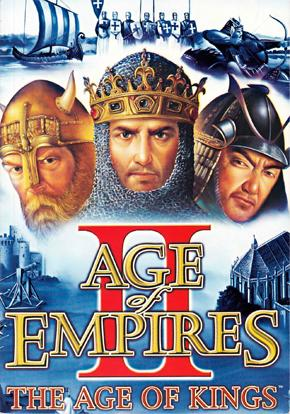
\includegraphics[width=0.3\textwidth]{imagenes/marco_teo/referentes/aoe_1.png}
\caption{Carátula del juego original.}
\label{img:aoe_1}
\end{figure}

En lo referente a edificaciones\footnote{Lista de edificios: \url{https://ageofempires.fandom.com/wiki/Buildings_(Age_of_Empires_II)}.}
podemos encontrar distintos tipos según su aporte al jugador,
el edifício printipal es el `Ayuntamiento' el cual nos permitirá crear colonos para que trabajen
recogiendo recursos y/o ayudando en la construcción de nuevas estructuras, en segundo lugar podemos
encontrar edifícios como el `Cuartel' o el `Campo de Tiro' los cuales nos permiten crear unidades
militares, por otro lado tenemos edificios como la `Herreria' la cual nos permitirá realizar investigaciones
y crear unidades de asedio.

Por último podemos encontrar estructuras de temática religiosa como el `Monasterio', otras 
destinadas a aumentar la productividad en la explotación de recursos naturales como el 
`Molino' y defensivas como la `Muralla'. 

\begin{figure}[ht]
\centering
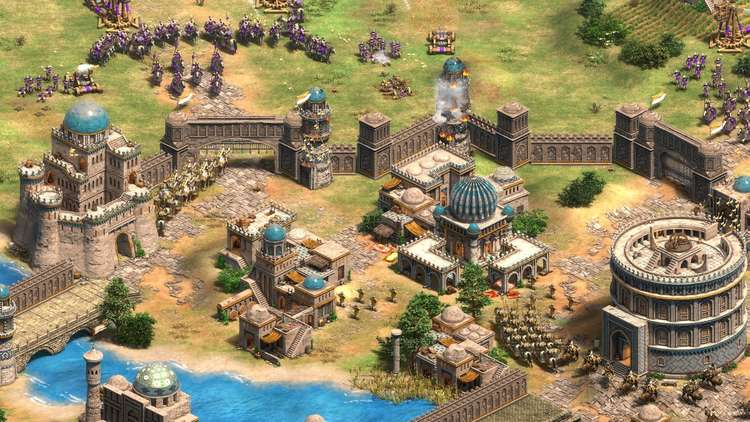
\includegraphics[width=0.7\textwidth]{imagenes/marco_teo/referentes/aoe_2.png}
\caption{Ciudad siendo asediada.}
\label{img:aoe_2}
\end{figure}

En el género \textit{\ac{RTS}} hay una tendencia al uso de una perspectiva isométrica con cámara fija
la cual solo podemos modificar haciendo \textit{zoom} o desplazandola por el entorno, esto seguramente
se deba a que es la configuración que mejor nos permite observar el mapa y todas las unidades que
hay en el. Además, el hecho de que sea fija nos libra de la problemática de ir ajustando la
cámara según la parte del mapeado que estemos, ya que, seguramente el mapeado y los elementos
visuales del juego también hayan sido diseñados teniendo esto en cuenta.

Como podemos ver en el artículo de \citeauthor*{Pritchard2000} sobre el desarrollo de \textit{\ac{AoE} 2},
la \ac{IA} del juego esta desarrollada completamente con un lenguaje de \textit{scripting} desarrollado
por ellos~\ref{img:aoe_scripting_1}, de esta forma el código consiste en una serie de constantes y variables definidas desde un
inicio y mediante condicionales realizar las acciones  y cambios pertinentes. Gracias a un usuario
de \textit{`GitHub'} podemos ver en las imagenes~\ref{img:aoe_scripting_2} el código usado en el juego
y confirmar como está elaborado.

\begin{figure}[ht]
\centering
\begin{minipage}[c]{0.45\linewidth}
	\hspace{20mm}
	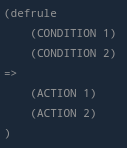
\includegraphics[height=0.15\textheight]{imagenes/marco_teo/referentes/aoe_scripting_1.png}
	\caption{Descripción Estructura.}
	\label{img:aoe_script_1}
\end{minipage}
\begin{minipage}[c]{0.45\linewidth}
	\hspace{9mm}
	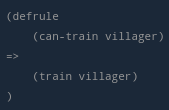
\includegraphics[height=0.15\textheight]{imagenes/marco_teo/referentes/aoe_scripting_2.png}
	\caption{Ejemplo condición.}
	\label{img:aoe_script_2}
\end{minipage}\\[3mm]
\textbf{Fuente:} guía de scripting para \ac{IA} de \ac{AoE} 2 de \citeauthor*{redmechanic2017}.
\label{img:aoe_scripting_1}	
\end{figure}

\begin{figure}[ht]
\centering
\begin{minipage}[c]{0.45\linewidth}
	\hspace{9mm}
	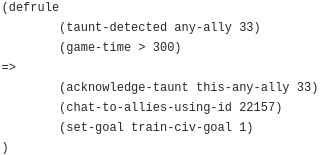
\includegraphics[height=0.11\textheight]{imagenes/marco_teo/referentes/aoe_scripting_3.png}
	\caption{Ejemplo condición.}
	\label{img:aoe_script_3}
\end{minipage}
\begin{minipage}[c]{0.45\linewidth}
	\hspace{2mm}
	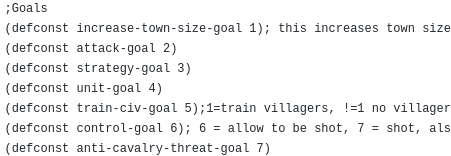
\includegraphics[height=0.11\textheight]{imagenes/marco_teo/referentes/aoe_scripting_4.png}
	\caption{Ejemplo constantes.}
	\label{img:aoe_script_4}
\end{minipage}\\[3mm]
\textbf{Fuente:} repositorio de \textit{'GitHub'} del usuario \citeauthor*{Andygmb2014}. 
\label{img:aoe_scripting_2}	
\end{figure}

Además de estos \textit{scripts} el juego utiliza un sistema de \textit{pathfinding} en dos niveles,
el primero de los algoritmos calcula la ruta a seguir por las unidades sin tener el cuenta los
elementos triviales como las demás unidades, mientras que la segunda pasada calcula el camino 
en tramos específicos con el fin de esquivar otras unidades, edificaciones, etc...

En lo referente al movimiento de las unidades, tanto por la forma en la que está programada
la \ac{IA} como por la sensación que dan al jugar, es posible que se trate de un  \textit{``Goto''}
clásico y sencillo para evitar realizar muchos cálculos. \\
Además, con el tiempo el juego se ha convertido en un objetivo para \textit{``Speedrunners''}
y con una escena competitiva que se basa en ser el más rápido jugando\footnote{En los enfrentamientos de alto rango se llegan a medir las acciónes por minuto (APM).}
por lo que una reacción instantánea de las unidades es un factor importante para  estos
jugadores.

\section{The Are Billions}
En segundo lugar podemos encontrar el juego \textit{'\acf{TaB}'} el cual se localiza en un
mundo postapocalíptico infestado de zombis donde quedan muy pocos superviventes, el juego
cuenta con dos modos:

En primer lugar encontramos el modo \textbf{horda} en el cual deberemos sobrevivir a
sucesivas oleadas de zombis, la cuales serán cada vez más grandes y con unidades más poderosas.
Además, deberemos mejorar nuestra colonia y sus defensas para poder lograr pasar las rondas.\\
En segundo lugar tenemos el modo \textbf{campaña}, el cual consistirá en una serie de misiones con el
fin de ampliar el tamaño de nuestro imperio a la vez que conocemos su historia y personajes
clave. 

\begin{figure}[ht]
\centering

\includegraphics[width=0.7\textwidth]{imagenes/marco_teo/referentes/tab_1.png}
\caption{Imágen promocional del juego.}
\label{img:tab_1}
\end{figure}

En \textit{'\ac{TaB}'} podemos ver como se reutilizan una serie de características propias
del género como pueden ser: el uso de una perspectiva isométrica con cámara fija o el uso de
un ``árbol tecnológico'' por el cual deberemos escalar si queremos desbloquear nuevas unidades
y/o mejorar las ya disponibles.

Si nos fijamos en las construcciones\footnote{Lista de edificios: \url{https://they-are-billions.fandom.com/wiki/Category:Buildings\#Buildings}.}
disponibles en el juego, encontramos como se sigue la línea de un ``Ayuntamiento'' como núcleo
de nuestra base, el cual nos permitirá conseguir trabajadores y nos dará acceso a las primeras
mejoras. Por otro lado, encontramos las edificaciones destinadas a conseguir recursos, reclutar
nuevas tropas y/o defender nuestra colonia. \\
En este juego se introduce como novedad el recurso de la `energía', el cual será utilizado
para mantener nuestras maquinárias en funcionamiento y nos limitará cuanto y donde podremos construir.  
Para ganar energía y ampliar el terreno disponible el jugador deberá construir `torres de Tesla' (o sus respectivas mejoras).


A diferencia de en \textit{'\ac{AoE}'}, en \textit{'\ac{TaB}'} encontramos la aparición de solamente dos facciones:
`El Nuevo Imperio', la facción del jugador, la cual representa una 
serie de colonias que tendremos que desarrollar a lo largo de los niveles, y en el otro lado, 
encontramos las infinitas hordas de zombis que tratarán de exterminar a la raza humana.

Cada una de las facciones tiene sus propias unidades~\ref{img:tab_2}, el jugador contará con 7 unidades distintas
entre las que podemos encontrar desde unas rápidas y sigilosas exploradoras hasta unidades equipadas
con lanzallamas o montados en robots de combate. \footnote{Lista unidades imperiales: \url{https://they-are-billions.fandom.com/wiki/Category:Units}.}
\\Las hordas enemigas estarán compuestas en su mayoria por unidades débiles que de forma eventual
serán acompañadas por gigantes~\ref{img:tab_3} y/o otras unidades especiales.
\footnote{Lista unidades zombi: \url{https://they-are-billions.fandom.com/wiki/Category:Infected}.}

\begin{figure}[ht]
\centering
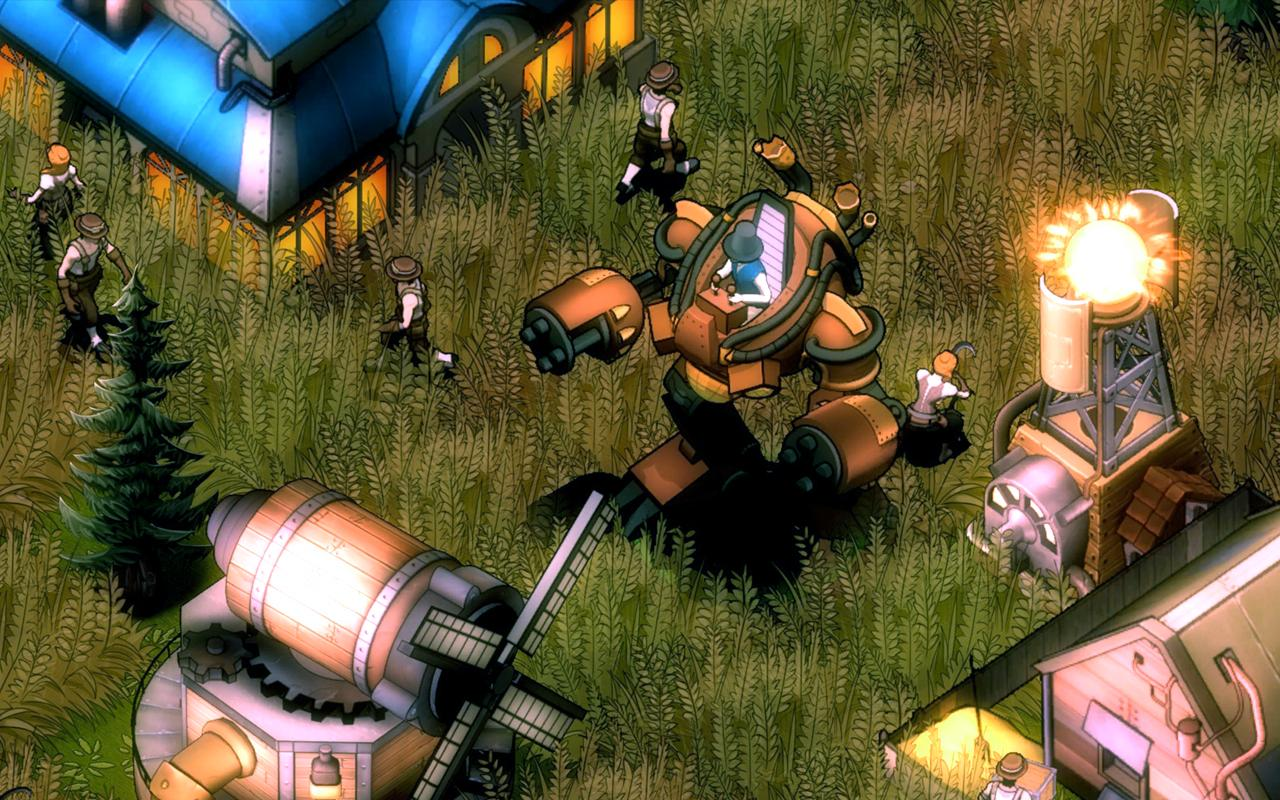
\includegraphics[width=0.6\textwidth]{imagenes/marco_teo/referentes/tab_2.png}
\caption{Ejemplo de elementos tecnológicos del juego.}
\label{img:tab_2}
\end{figure}

\begin{figure}[ht]
\centering
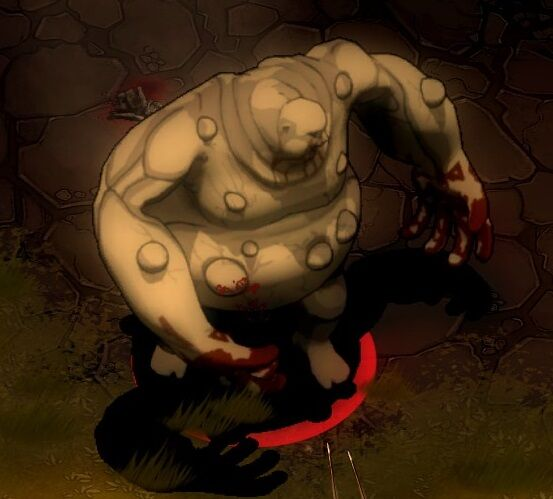
\includegraphics[width=0.4\textwidth]{imagenes/marco_teo/referentes/tab_3.png}
\caption{Infectado gigante}
\label{img:tab_3}
\end{figure}

A lo largo del juego podemos encontrar funciones interesantes e inovadoras como la pausa
táctica, la cual nos permitirá visualizar detenidamente el estado del mapa sin tener que
preocuparnos por no estar atendiendo algunos posibles eventos, como ataques a nuestras
tropas por parte del enemigo.\\ 
En juegos anteriores como los \textit{'\ac{AoE}'} es
fácil encontrarnos en la situación de tener trabajadores en la ciudad sin hacer tareas
un rato y, no poder mirar cuales son e ir pensando su ocupación siguiente por estar
atrapados en refriegas con otros jugadores, con este tipo de mecánicas estas situaciones
se solventan en mayor o menor medida y permiten al jugador tomarse el tiempo que
necesite para pensar las acciones que quiere realizar.

Otra adición interesante es la posibilidad de hacer una captura de todo el mapeado explorado~\ref{img:tab_4}
en el nivel pudiendo así mostrar el avance de nuesta ciudad y alrededores, además de la 
inmensidad de las oleadas de zombis que nos irán atacando.

\begin{figure}[ht]
\centering
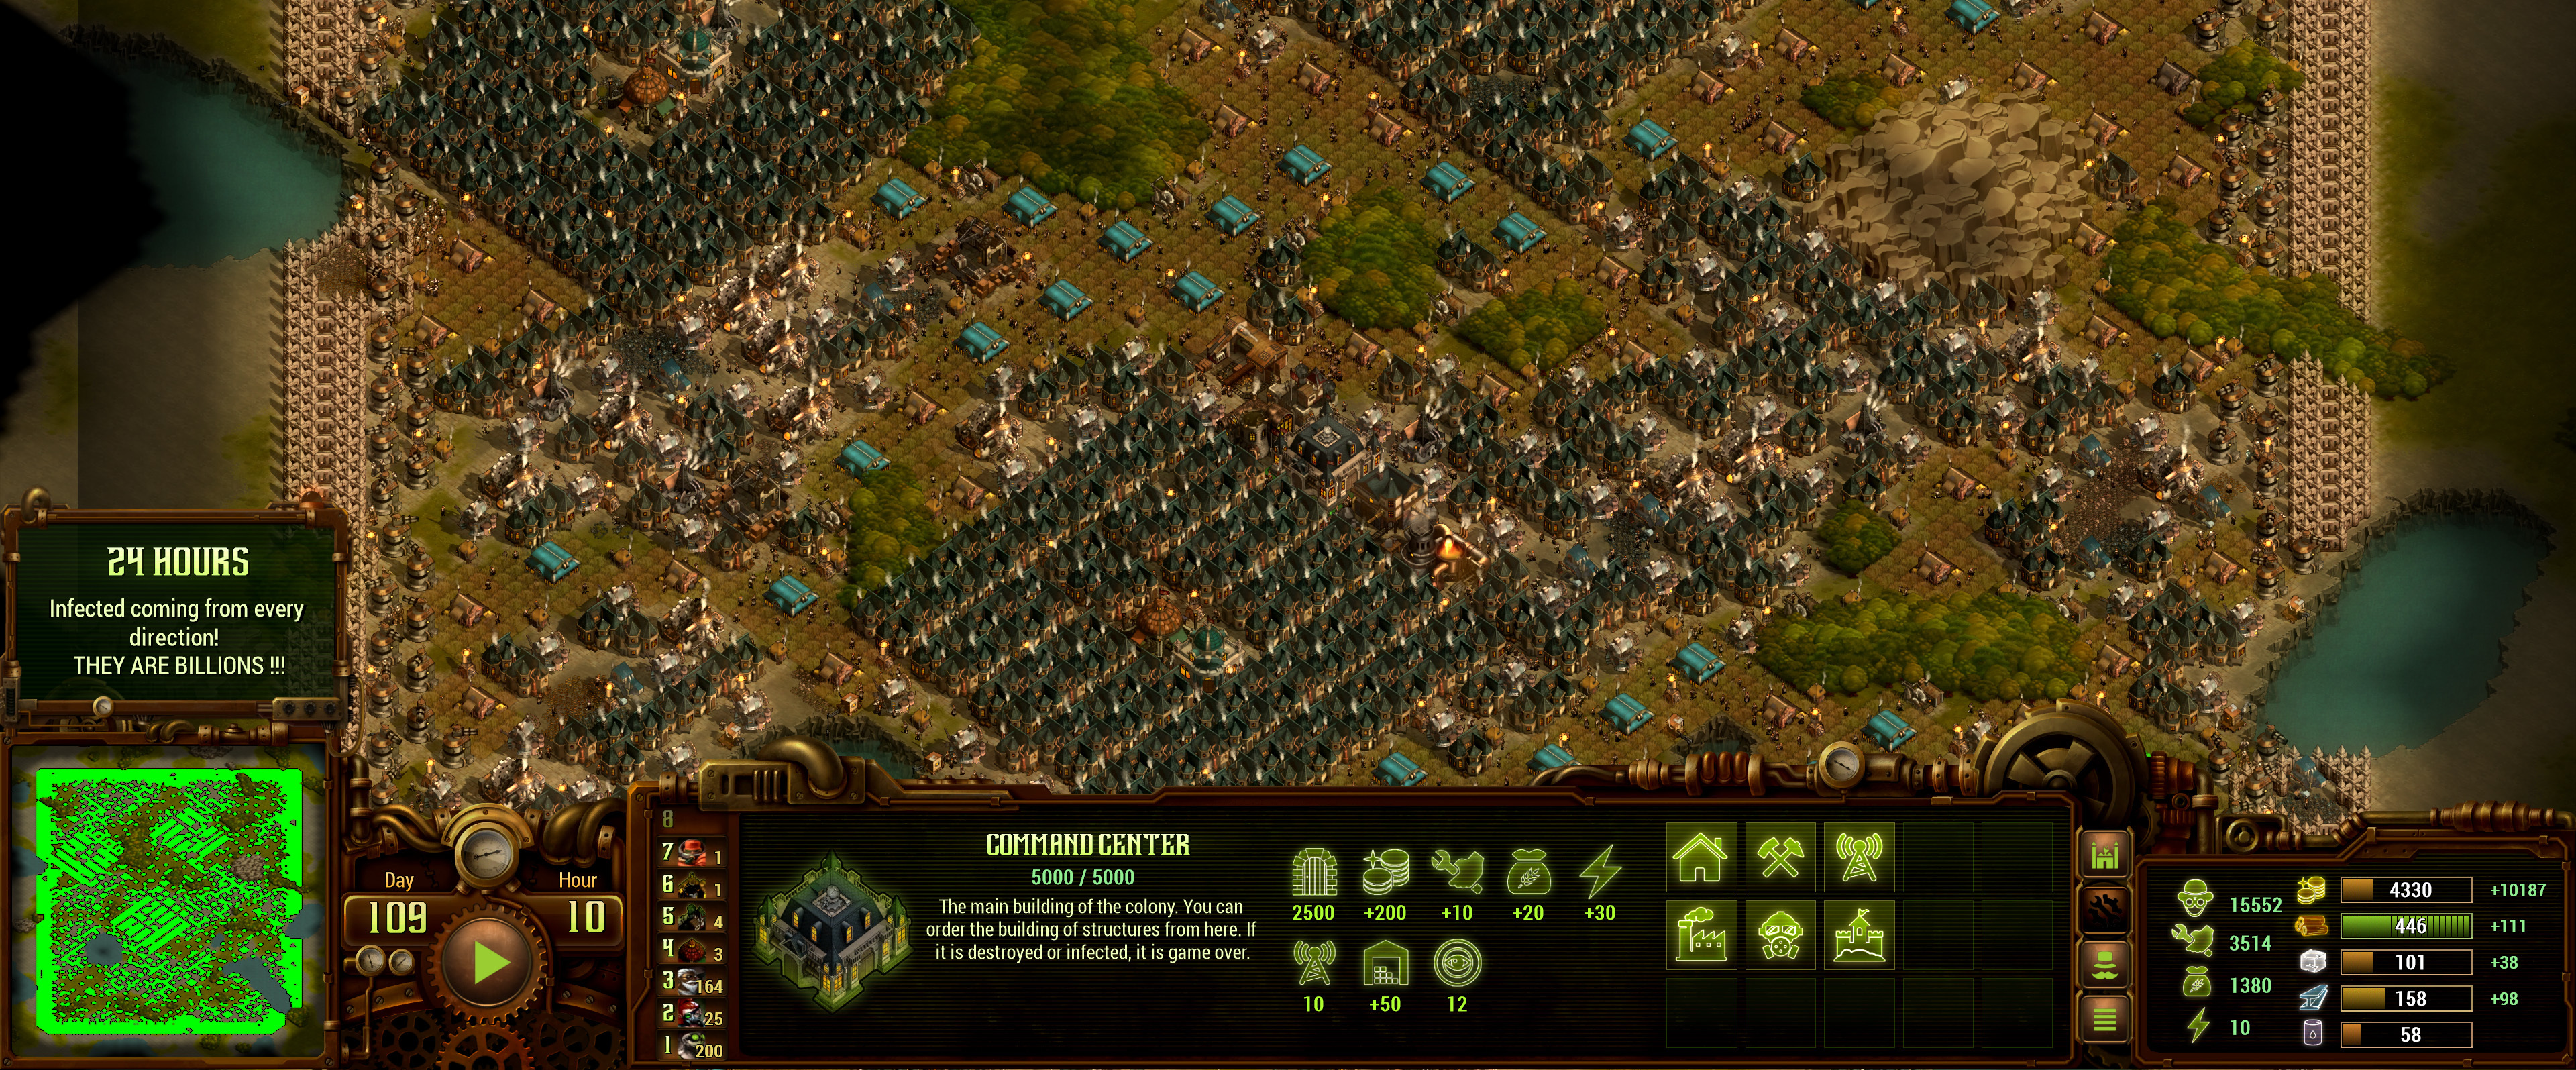
\includegraphics[width=0.7\textwidth]{imagenes/marco_teo/referentes/tab_4.png}
\caption{Ejemplo de captura global del nivel.}
\label{img:tab_4}
\end{figure}

En lo refente a la \ac{IA}, podemos observar como intentan replicar la forma de actuar del
zombi común. Como podemos leer en la entrevista a `Jesús Arribas' y `Miguel Corral'
\footnote{Responsables principales de Numantian Games y desarrolladores del juego.} por parte
de \citeauthor*{Sucasas2018} para el portal `Xakata', cada zombi cuenta con mecanismos para 
detectar a los humanos, ya sea por divisarlos visualmente o escucharlos moverse, además si un 
compañero cercano ha encontrado un objetivo, este le seguirá siguiendo 
una mentalidad de manada a la que se irán sumando los zombis en su recorrido.

Mientras los infectados estén sin un objetivo específico, pueden darse dos escenarios:
el primero nos muestra enemigos dispersos por el mapa esperando a que el jugador se aventure
a explorar esa zona y sorprenderle con un ataque. El otro nos trae las oleadas que aparecen
en los límites del mapa las cuales tienen como objetivo el centro de nuestra base, si los
enemigos estáticos por el mapa divisan la horda se unirán a ella aumentando así su poder, esto
sin duda alienta al jugador a ``limpiar'' el mapa con el fin de aliviar estas acometidas.\\
Como la intención de la \ac{IA} es la de replicar la forma de ``no pensar'' de los zombis, en
el momento en que unidades humanas se presenten delante de las hordas de enemigos estos se
dispondrán a perseguir a estas personas, perdiendo así el foco en nuestra base. Esto abre las
puertas a poder jugar con el \textit{``aggro''} de los zombis de forma estratégica.

En paralelo a las declaraciones de los \textit{devs}, parte de la comunidad discutía sobre si
la \ac{IA} del juego hacía trampas con tal de incrementar la dificultad, a lo que el usuario
\citeauthor*{Steam_User2019} comenta las declaraciones de los desarrolladores y niega que la
máquina haga trampas, para apoyar sus palabras nos redirije a un \textit{post} de \textit{`Reddit'}
donde \citeauthor*{Pikachunet2018} nos muestra capturas de un posible editor de niveles del
juego en el que se nos muestran multitud de opciones, entre las que encontramos la cantidad de
enemigos, como se disponen en el mapa, o si tendrán esa iniciativa de ir al centro de la base.


\section{Sea Salt}
Como podemos observar en los anteriores referentes, dentro del género \ac{RTS} da la sensación
de que todos los recursos destinados a \ac{IA} estaban reservados para la toma de decisiones y 
en gestionar la civilización, dejando el desplazamiento de las unidades y el combate como algo
trivial. \\
Dicho sea que el género nació cuando no había casi capacidad de procesamiento
y ,con el paso del tiempo, el hecho de intentar consevar la esencia del género a ocasionado la
herencia de experiencias de juego un ``poco básicas``.

\begin{figure}[ht]
\centering
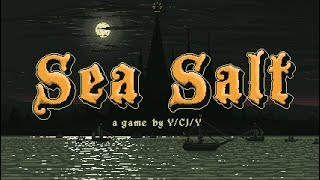
\includegraphics[width=0.7\textwidth]{imagenes/marco_teo/referentes/ss_1.png}
\caption{Menú principal}
\label{img:ss_1}
\end{figure}

Por otro lado, hay juegos que han aportado experiencias y mecánicas nuevas, ya sea combinando
géneros y/o incluyendo técnicas más modernas que nos ofrecen resultados distintos. Este es el
caso de \textit{`Sea Salt'}, juego que combina estrategia, acción y cartas en el que encarnaremos 
a `Dagon' una antigua deidad marina la cual planea castigar a la humanidad por haberse 
opuesto a sus designios.

El juego se compone de una serie de niveles que representan distintas partes de la ciudad
donde se desarrolla la historia, cada nivel tiene a su vez distintas salas donde encontraremos
diversos obstáculos y enemigos que abatir. Para abrirnos paso por el nivel manejaremos al
ejercito de `Dagon' el cual se compone de diversas criaturas cada una con sus carácteristicas 
únicas, a lo largo de los niveles encontraremos altares donde podremos invocar nuevas unidades
para aumentar el grueso de nuestras filas. 

En este caso los puntos que más nos interesa tratar es el uso de \textit{`Flocking'} y el 
control de las unidades que controla el jugador.

\begin{figure}[ht]
\centering
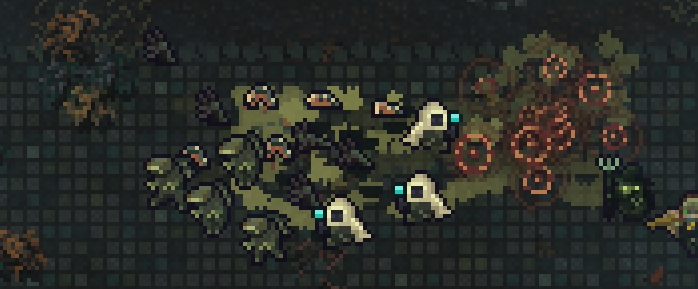
\includegraphics[width=0.7\textwidth]{imagenes/marco_teo/referentes/ss_4.png}
\caption{Criaturas de `Dagon'}
\label{img:ss_4}
\end{figure}

En cuanto a la jugabilidad y los controles, el jugador no manejará de forma
explícita las criaturas del ejercito, sino que, mediante las teclas `w', `a', `s', `d'
moverá una marca por el mapa la cual será seguida por las unidades. Además, con la
`barra espaciadora' las unidades se lanzarán al ataque de los enemigos en su rango de 
acción, aparentemente al más cercano. Por último encontramos la tecla `ctrl' la cual
nos permitirá hacer que las unidades se reagrupen en la marca del jugador y el `shift'
el cual 
hará que todas las unidades avancen a la misma velocidad. \\
Mediante estas acciones tendremos que arreglarnos las para matar a la unidades enemigas y
esquivar sus ataque, sobretodo en las peleas con jefes al final de los niveles.

Por otro lado encontramos el uso de \textit{'Flocking'} el cual aporta un toque ``errático''
en el desplazamiento de las unidades que, junto a los controles, juega mucho con la temática 
de monstruos/criaturas malvadas. \\
La técnica ayuda a darle vida y sensación de individualidad
a cada una de las unidades, a la vez que refuerza la visión de conjunto al ver como las
unidades se encuentran en todo momento actuando de la misma forma. 


\section{Técnicas de inteligencia articificial}
Como ha sido mencionado en la introducción~\ref{intro}, uno de los objetivos más importantes 
del proyecto recaen en el desarrollo de una \ac{IA} haciendo uso de las técnicas de 
\textit{'Flocking'} y \textit{`Steering behaviors'}.

Para ello nos basaremos principalmente en las explicaciones y ejemplos que podemos
encontrar en el libro \cite[ch.~3]{Millington2009} donde de forma extensa y detallada
se nos introduce en la teoría relacionada a los algoritmos y la forma en la que estos
se estructuran e interactuan entre ellos. Para dar un poco de contexto sobre el tema
resumiremos brevemente las ideas que se nos presentan a lo largo del capitulo dedicado
a estas técnicas. 

Los \textit{`Steering behaviors'} pueden ser entendidos como una serie de algoritmos
destinados a guiar la forma en la cual los \ac{NPC} se desplazan por el escenario
y/o interactuan con los distintos elementos que puedan encontrase en la escena. Siguen
una filosofía de crear movimientos complejos a base de una combinación de movimientos 
y/o acciones simples, un ejemplo común puede ser la acción de perseguir a un objetivo
mientras se sortean obstáculos en el proceso. \\ 
En este caso no tendríamos una función llamada 
\textit{``persigue-enemigo-mientras-esquivas()''} y esta encargarse de todo el 
trabajo, sino que, tendremos el cálculo de la velocidad y dirección necesarias para
alcanzar el objetivo, la compropación para saber si hay algún tipo de
obstáculo por el camino y la rectificación de la trayectoria en caso de
haberlos cada uno por su lado y es la resultante de todos los pasos la que defina el
movimiento final.

Esta forma de estructurar y formar actividades complejas en base a acciones más simples
nos permite reutilizar y jugar con los diferentes comportamientos permitiéndonos crear
con ellos un amplio espectro de resultados.

En lo referente al \textit{'Flocking'} podemos observar como en esencia es lo mismo que
los \textit{`Steering behaviors'} pero añadiendo factores y/o componentes grupales,
el origen del modelo lo podemos encontrar en las publicaciones de \cite{Boids1986} donde
se nos introduce el concepto de \textit{``Boid''} como entidad generica que simula su
comportamiento bajo este algoritmo. Además, se nos introducen los tres comportamientos
básicos en los que se basa la técnica para generar el movimiento emergente, que son:

La \textbf{separación}~\ref{img:separation-b} que cada \textit{Boid} mantendrá entre
las demás entidades en su vencidad, con esto evitaremos solapamientos y respetar el
espacio y movimiento de las demás entidades.

\begin{figure}[ht]
\centering
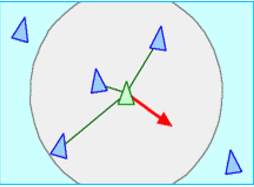
\includegraphics[width=0.35\textwidth]{imagenes/marco_teo/separation.png}
\caption{Separation behavior}
\label{img:separation-b}
\end{figure}

Por otro lado podemos encontrar el \textbf{alineamiento}~\ref{img:alignment-b} de la
dirección del movimento propio con las de las entidades más cercanas, de esta forma conseguimos un
movimiento armónico entre los \textit{boids} y produciremos una sensación de
coordinación entre ellos.

\begin{figure}[ht]
\centering
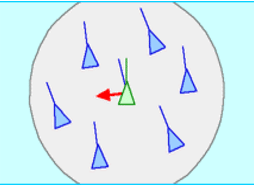
\includegraphics[width=0.35\textwidth]{imagenes/marco_teo/alignment.png}
\caption{Alignment behavior}
\label{img:alignment-b}
\end{figure}

Por último encontramos la \textbf{cohesión}~\ref{img:cohesion-b} la cual se encargará de
mantener a las entidades cercanas juntas para crear esa sensación de grupo que buscamos
con el algoritmo.

\begin{figure}[ht]
\centering
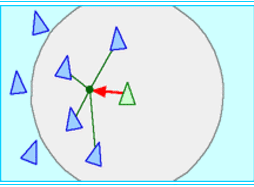
\includegraphics[width=0.35\textwidth]{imagenes/marco_teo/cohesion.png}
\caption{Cohesion behavior}
\label{img:cohesion-b}
\end{figure}

Por otro lado, podemos ver en el articulo de `Raynolds' como a lo largo de los años se
ha ido modificando y ampliando el algoritmo con el fin de añadir variaciones en el
comportamiento y/o introducir más factores influyentes en la decisión de los 
\textit{Boids} como puede ser el olor de determinada entidad/es y/o escenario. \\
Esto sin duda es gracias a la versatílidad que nos proporciona el uso de los
\textit{`Steering behaviors'} y jugar con la importancia de las distintas componentes
a la hora de hacer la toma de decisiones.

